% DPF 09 talk on strangeness in nucleon

\documentclass[10pt]{beamer}
\usefonttheme{professionalfonts} % using non standard fonts for beamer
\usefonttheme{serif} % default family is serif
\usepackage{amsmath}
\usepackage{mathtools}
\usepackage{mwe}
%\documentclass[12pt]{beamerthemeSam.sty}
\usepackage{epsf}
%\usepackage{pstricks}
%\usepackage[orientation=portrait,size=A4]{beamerposter}
\geometry{paperwidth=160mm,paperheight=120mm}
%DT favorite definitions
\def\LL{\left\langle}	% left angle bracket
\def\RR{\right\rangle}	% right angle bracket
\def\LP{\left(}		% left parenthesis
\def\RP{\right)}	% right parenthesis
\def\LB{\left\{}	% left curly bracket
\def\RB{\right\}}	% right curly bracket
\def\PAR#1#2{ {{\partial #1}\over{\partial #2}} }
\def\PARTWO#1#2{ {{\partial^2 #1}\over{\partial #2}^2} }
\def\PARTWOMIX#1#2#3{ {{\partial^2 #1}\over{\partial #2 \partial #3}} }

\def\rightpartial{{\overrightarrow\partial}}
\def\leftpartial{{\overleftarrow\partial}}
\def\diffpartial{\buildrel\leftrightarrow\over\partial}

\def\BI{\begin{itemize}}
\def\EI{\end{itemize}}
\def\BE{\begin{displaymath}}
\def\EE{\end{displaymath}}
\def\BEA{\begin{eqnarray*}}
\def\EEA{\end{eqnarray*}}
\def\BNEA{\begin{eqnarray}}
\def\ENEA{\end{eqnarray}}
\def\EL{\nonumber\\}


\newcommand{\map}[1]{\frame{\frametitle{\textbf{Course map}}
\centerline{\includegraphics[height=0.86\paperheight]{../../map/#1.png}}}}
\newcommand{\wmap}[1]{\frame{\frametitle{\textbf{Course map}}
\centerline{\includegraphics[width=0.96\paperwidth]{../../map/#1.png}}}}

\newcommand{\etal}{{\it et al.}}
\newcommand{\gbeta}{6/g^2}
\newcommand{\la}[1]{\label{#1}}
\newcommand{\ie}{{\em i.e.\ }}
\newcommand{\eg}{{\em e.\,g.\ }}
\newcommand{\cf}{cf.\ }
\newcommand{\etc}{etc.\ }
\newcommand{\atantwo}{{\rm atan2}}
\newcommand{\Tr}{{\rm Tr}}
\newcommand{\dt}{\Delta t}
\newcommand{\op}{{\cal O}}
\newcommand{\msbar}{{\overline{\rm MS}}}
\def\chpt{\raise0.4ex\hbox{$\chi$}PT}
\def\schpt{S\raise0.4ex\hbox{$\chi$}PT}
\def\MeV{{\rm Me\!V}}
\def\GeV{{\rm Ge\!V}}

%AB: my color definitions
%\definecolor{mygarnet}{rgb}{0.445,0.184,0.215}
%\definecolor{mygold}{rgb}{0.848,0.848,0.098}
%\definecolor{myg2g}{rgb}{0.647,0.316,0.157}
\definecolor{abtitlecolor}{rgb}{0.0,0.255,0.494}
\definecolor{absecondarycolor}{rgb}{0.0,0.416,0.804}
\definecolor{abprimarycolor}{rgb}{1.0,0.686,0.0}
\definecolor{Red}           {cmyk}{0,1,1,0}
\definecolor{Grey}           {cmyk}{.7,.7,.7,0}
\definecolor{Lg}           {cmyk}{.4,.4,.4,0}
\definecolor{Blue}          {cmyk}{1,1,0,0}
\definecolor{Green}         {cmyk}{1,0,1,0}
\definecolor{Brown}         {cmyk}{0,0.81,1,0.60}
\definecolor{Black}         {cmyk}{0,0,0,1}

\usetheme{Madrid}
\newcommand{\vcenteredinclude}[1]{\begingroup
  \setbox0=\hbox{\includegraphics[width=3in]{#1}}%
\parbox{\wd0}{\box0}\endgroup}

%AB: redefinition of beamer colors
%\setbeamercolor{palette tertiary}{fg=white,bg=mygarnet}
%\setbeamercolor{palette secondary}{fg=white,bg=myg2g}
%\setbeamercolor{palette primary}{fg=black,bg=mygold}
\setbeamercolor{title}{fg=abtitlecolor}
\setbeamercolor{frametitle}{fg=abtitlecolor}
\setbeamercolor{palette tertiary}{fg=white,bg=abtitlecolor}
\setbeamercolor{palette secondary}{fg=white,bg=absecondarycolor}
\setbeamercolor{palette primary}{fg=black,bg=abprimarycolor}
\setbeamercolor{structure}{fg=abtitlecolor}

\setbeamerfont{section in toc}{series=\bfseries}

%AB: remove navigation icons
\beamertemplatenavigationsymbolsempty
\title{
  \textbf {Resonant modes in interesting shapes}\\
%\centerline{}
%\centering
%\vspace{-0.0in}
%\includegraphics[width=0.3\textwidth]{propvalues_0093.pdf}
%\vspace{-0.3in}\\
%\label{intrograph}
}

\author[W. Freeman] {Physics 211\\Syracuse University, Physics 211 Spring 2017\\Walter Freeman}

\date{\today}

\begin{document}

\frame{\titlepage}

\frame{\frametitle{\textbf{Announcements}}
  \large
\BI
\item{Please be patient with TA's while they process exam corrections}
\item{If they don't get to evaluate yours in person, they can look at your written version}
\item You must be in recitation on Friday to do exam corrections 
\item If you have a medical or emergency reason for missing recitation Friday, you can come to office hours and do them
\pause
\BI
\normalsize
\item Mayfest is not an excused absence; classes are still in session Friday
\pause
\item Do not show up drunk to recitation (it won't end well)
\pause
\EI
\item Extra clinic hours ahead of the final exam: 
\BI
\normalsize
\item 10AM-4PM next Wednesday
\item Review sessions TBD -- probably next Thursday and Sunday, at least
\EI
\EI
}



\frame{\frametitle{\textbf{Standing waves, from before}}
  \Large
  \vcenteredinclude{mode1-crop.pdf} Fundamental: $f_1 = \frac{c}{2L}$\\
 \bigskip 
  \vcenteredinclude{mode2-crop.pdf} 2nd harmonic: $f_2 = 2 f_1 $\\
 \bigskip 
  \vcenteredinclude{mode3-crop.pdf} 3rd harmonic: $f_3 = 3 f_1$ \\
  
 \bigskip 
  \vcenteredinclude{mode4-crop.pdf} 4th harmonic: $f_4 = 4 f_1$ \\
  
 \bigskip 

}

\frame{\frametitle{\textbf{Musical instruments: fun with spectroscopy}}
  \large
  \BI
\item{In general, when you excite a string or air column, you produce a combination of many standing wave modes}
\item{The unique sound of each instrument comes mostly from the relative strengths of them}
  \BI
\item{``Dark'' or ``pure'' sound: weak higher harmonics}
\item{``Bright'' or ``brassy'' sound: strong higher harmonics}
  \EI
\item{All of these pitched instruments have evenly-spaced frequencies}
\item The unique sound of each instrument is determined by which frequencies are strongest
\item{This is necessary for something to sound like a musical note}
\item{Strings and uniform tubes do this naturally}
  \EI
}

\frame{\frametitle{\textbf{Interesting shapes}}
\Large

What frequencies do we expect from an object of a complex shape?

\bigskip

\BI
\item A: An evenly-spaced set of frequencies: a fundamental and integer multiples
\item B: Frequencies in the pattern $f,\,3f,\,5f,\,7f,\,9f...$
\item C: Just one frequency
\item D: Many frequencies in a complicated pattern (horizontal lines unevenly spaced)
\item E: A continuous band of frequencies (a vertical line, or a blob)
\EI
}



\frame{\frametitle{\textbf{A simple example: the xylophone and its cousins}}
\large
Instrument made from wooden bars: small ones are high notes, big ones are low notes

\bigskip
\centerline{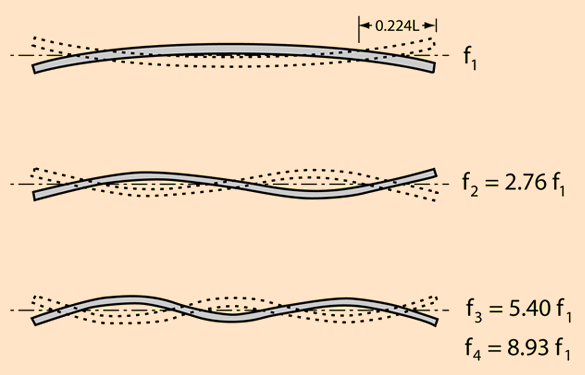
\includegraphics[width=0.5\textwidth]{bar-modes.png}}
\bigskip
Our metal bar works like this. What does it sound like?
\pause
\bigskip

We have a problem: the frequencies of the normal modes are {\it not harmonic!}; they don't form ratios of 1, 2, 3, 4...
\normalsize
\BI
\item{If these are allowed to vibrate, the instrument won't sound like a single musical pitch}
\pause
\item{Solution: support the bar at the nodes of the first mode}
\item{This allows that mode to vibrate, but damps out the others that don't have nodes there}
\item{The peculiar sound of the marimba comes from the rapid decay of these non-harmonic modes}
  \EI
}

\frame{\frametitle{\textbf{Normal modes for other shapes}}
  \large
\BI
\item{In general, other shapes have a huge diversity of vibrational modes!}
\item{A few examples...}
  \pause
\item{Simulations:}
  \BI
\large
\item{Circular membrane: like a drumhead. How does it resonate/move?}
  \EI
\item{Real examples}
  \BI
\large
\item{Chladni plates}
\item{Other fancy toys...}
  \EI
  \EI
}

\frame{\frametitle{\textbf{Far more than just acoustics!}}
  \large
  \BI
\item{These ideas of resonance and normal modes apply to {\it anything} that can oscillate!}
\item{Key ideas:}
  \BI
\large
\item{An object can vibrate in particular ways determined by its structure}
\item{Each of those {\bf normal modes} has a particular frequency}
\item{It absorbs energy very readily at those frequencies}
  \EI
\item{Electric circuits: antennas (standing waves in a wire!), and the equivalent of masses on strings}
\item{Mechanical designs of all sorts of things}
  \pause
\item{Architecture: {\color{Red} \bf resonance is very bad...}}
  \pause
\item{Lots of work goes into ensuring that there are no strong resonances where there shouldn't be any...}
  \EI
}

  \frame{\frametitle{\textbf{Quantum mechanics and the connection to chemistry}}
    \centerline{\Large\color{Red} A key idea in quantum mechanics: matter acts like a wave}
    \large
    \BI
  \item{Are there normal modes for atoms, too?}
    \pause
  \item{You bet! These standing wave patterns (for matter waves) are the orbitals you study in chemistry!}
\item In QM, differences in energy correspond to a frequency: $f = E / h$
    \EI
  \bigskip
  \bigskip
  \centerline{  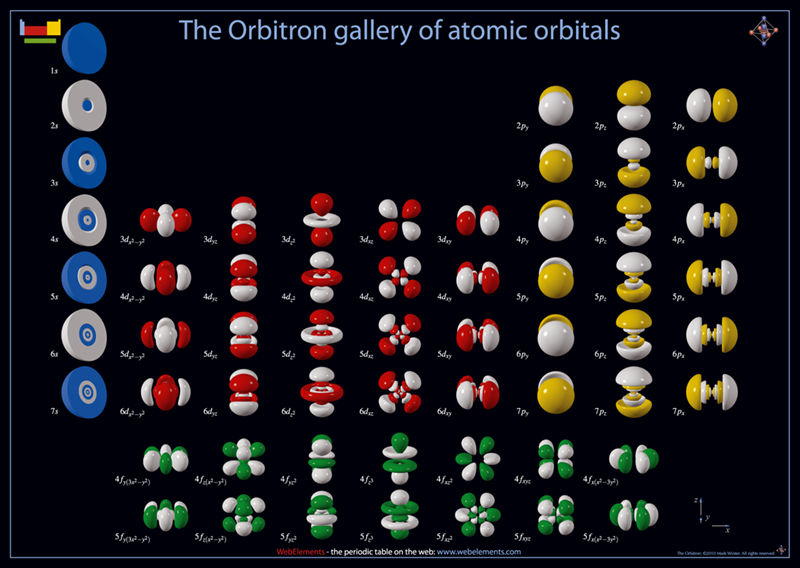
\includegraphics[width=0.55\textwidth]{orbitals.jpg}}
  \bigskip
  \bigskip
  \centerline {\normalsize  Great advances in quantum mechanics were made by people thinking about violin strings!}
}

\frame{\frametitle{\textbf{Resonance appears everywhere...}}
  \large
  \BI
\item{Studying the resonant modes of molecules can tell us a great deal!}
\item{Every molecule has certain resonant frequencies}
  \BI
\item{Think of the mechanics of molecular bonds flexing...}
\item{This involves the combination of the laws of motion you learned here, plus quantum mechanics}
  \EI
\EI
}

\frame{\frametitle{\textbf{Resonance appears everywhere...}}
\Large
You're a radio astronomer examining a cloud of dust between the stars. You detect a certain set of 
frequencies coming from it. What do you do?

\bigskip
\centerline{Raise your hand and make suggestions!} 
\bigskip

\pause
\BI
\large
\item{``Light'', too, is a wave}
\item{We can study strings by looking at how they couple to sound waves...}
\item{... physicists and chemists study atoms and molecules by looking at how they couple to light waves!}
\item Previously: ``I know the shape: let me calculate the resonant frequencies''
\item This works in reverse: if I know the resonant frequencies, maybe I can find the shape?
\EI

\large\bigskip

We've measured the resonant frequencies of glycine, an amino acid, in the lab.

Radio astronomers have detected that same set of frequencies coming from space...

 ... with just an antenna and some math, we have found organic molecules between the stars! 

}

\frame{\frametitle{\textbf{Looking at the Sun}}
\Large
\begin{center}
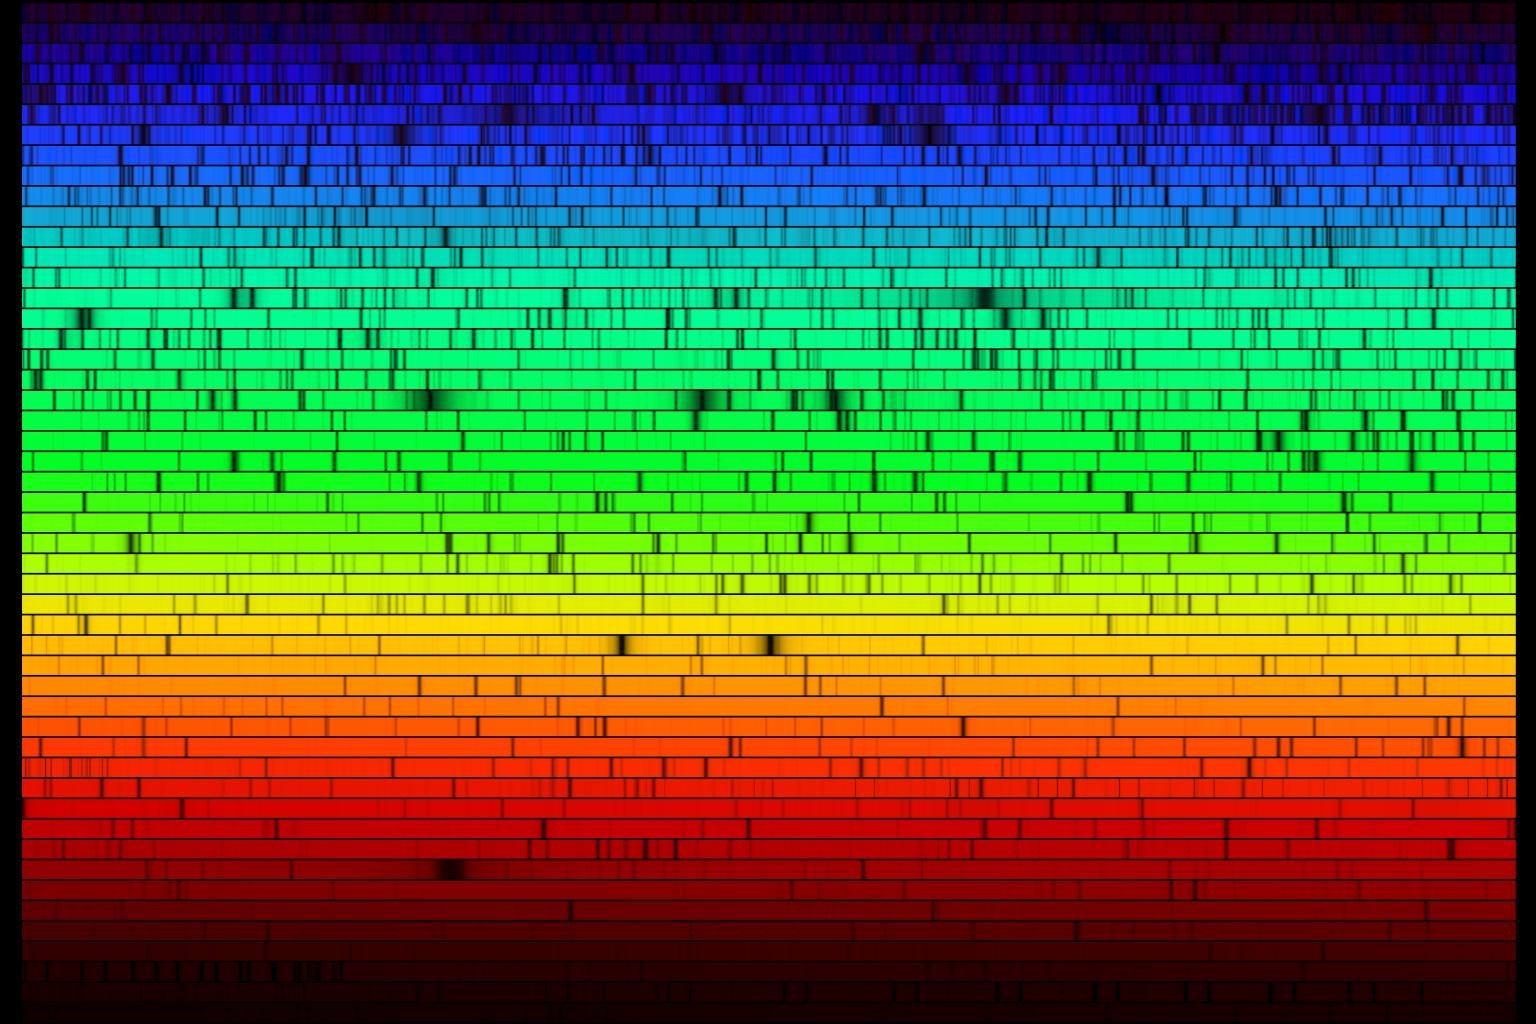
\includegraphics[width=0.9\textwidth]{sun-spectrum.jpg}

\bigskip

What do these lines tell you about the Sun?

\end{center}
}

\frame{\frametitle{\textbf{Looking at the Sun}}
\Large
You discover lines in the solar spectrum that don’t correspond
to any known element. What do you conclude?

\bigskip
\BI

\item A: Something about quantum mechanics is different in the Sun
\item B: Something about light is different in the Sun
\item C: There's an element in the Sun that’s not on Earth -- call it
{\bf sunium}
\item D: The extreme temperature of the Sun causes new lines to
appear in its gas
\item E: All of those seem not right, and ``sunium" isn't on the periodic table
\EI
}

\frame{\frametitle{\textbf{Resonance appears everywhere...}}
\Large
\BI
\item{Going even smaller, particle physicists do the same thing: we even mix up the words!}
\item Highly unstable particles are called ``resonances''
\item{You might even say: most of science appears in the concert hall!}
\EI
}

\frame{\frametitle{\textbf{The power of mechanics}}
\large
The things we've studied in this class are more powerful than you think. 

If you call up a chemist, she'll tell you the approximate force law between two noble gas atoms:

$$ F(r) = \frac{\alpha}{r^12} - \frac{\beta}{r^6} $$

Put this into a computer and let it go:

\pause\bigskip

\centerline{\color{Red}We can understand freezing, melting, and boiling just with $\vec F = m \vec a!$}

\centerline{\color{Red}... we can even get the ideal gas law for free along the way!}
}

\frame{\frametitle{\textbf{The rest of physics}}
\large
The other disciplines of physics are variants on what you've learned already:

\BI
\item Electromagnetism (PHY 211) introduces a new force -- just another $\vec F$
\BI
\item Light is just a particular manifestation of that force
\EI
\item Statistical mechanics uses statistics to understand 
$\vec F = m\vec a$ acting on a great many particles at once
\item Relativity mixes up space and time, changing the coordinates on us
\item Quantum mechanics mixes up ``particle'' and ``wave''
\EI

Each of these disciplines is supported by a ``three-legged stool'':

\BI
\item Theory: understanding principles and using pen and paper to study them in simple situations (this class)
\item Experiment: designing tests for these principles and building machines to carry them out (221)
\item Computation: using computers to simulate those principles in more complicated situations and study their consequences (my field and class in the fall)
\EI
}

\frame{\frametitle{\textbf{I leave you with two quotes...}}
\pause
``A poet once said, 'The whole universe is in a glass of wine.'...  [I]f we look at a glass of wine closely enough we see the entire universe. 
There are the things of physics: the twisting liquid which evaporates depending on the wind and weather, the reflection in the glass; and our imagination adds atoms. 
The glass is a distillation of the earth's rocks, and in its composition we see the secrets of the universe's age, and the evolution of stars. 
What strange array of chemicals are in the wine? 
How did they come to be?... 
If our small minds, for some convenience, divide this glass of wine, this universe, into parts -- physics, biology, geology, astronomy, psychology, 
and so on -- remember that nature does not know it! So let us put it all back together, not forgetting ultimately what it is for. Let it give us one more final pleasure; drink it and forget it all!''

\bigskip
\bigskip

\pause

``Poets say science takes away from the beauty of the stars — mere globs of gas atoms. Nothing is "mere". I too can see the stars on a desert night, and feel them. But do I see less or more? The vastness of the heavens stretches my imagination — stuck on this carousel my little eye can catch one-million-year-old light. A vast pattern — of which I am a part... What is the pattern, or the meaning, or the why? It does not do harm to the mystery to know a little about it. For far more marvelous is the truth than any artists of the past imagined!''

\bigskip

--Richard Feynman, from {\em Lectures on Physics}
}
\end{document}
